% !TEX encoding = UTF-8
% !TEX TS-program = pdflatex
% !TEX root = computabilità e algoritmi.tex
% !TEX spellcheck = it-IT
\subsubsection{Esercizio - Tandem massimale}\label{esercizio---tandem-massimale}

Nelle sequenze biologiche è importante riconoscere eventuali ripetizioni consecutive della stessa sottostringa.
Una tale sequenza di ripetizione di una sottostringa \textit{A} in una stringa \textit{T} viene detta \textbf{tandem array} di \textit{A}.

Ad esempio la stringa \textit{T = cdabcabcabcabcxga} contiene  il tandem array \textit{abcabcabcabc} di \textit{A = abc} di lunghezza 4.
Un tandem array è massimale se non può essere esteso né a destra né a sinistra.

Data la base \textit{A}, un tandem array di \textit{A} in \textit{T} può essere può essere individuato da una coppia di numeri \textit{(s,k)} in cui \textit{s} indica la posizione nel testo \textit{T} dove inizia il tandem array e \textit{k} è il numero di ripetizioni di \textit{A}.

Descrivere un algoritmo che dato un testo \textit{T} e una stringa \textit{A} non periodica, calcola in tempo lineare tutti i tandem array di \textit{A} massimali fornendo in output le corrispondenti coppie \textit{(s,k)}.



\paragraph{Soluzione}\label{soluzione}

Si concatenano \emph{A} e \emph{T} in modo da formare \emph{S = A\$T} e si calcolano i vari $\pi_i$ in modo da trovare le occorrenze del
pattern.

Se $\pi_j$ è un occorenza di \emph{A}, si va a controllare
$\pi_j+len(A)$ e così via, finché non ci sono più occorrenze in
fila.

Può essere che i pattern si sovrappongano al più per qualche carattere,
quindi quando viene trovato l'ultimo elemento dell'array, è necessario
controllare anche i vari $\pi_j$ precedenti, per verificare che non ci sia un altro tandem array.

Non è necessario controllare i $\pi_j$ intermedi ad un tandem array,
perché dal momento che la stringa \emph{A} non è periodica, non può
esserci un'occorrenza di \emph{A} a cavallo tra altre due occorrenze di
\emph{A}.

\section{Algoritmi base per il pattern matching}\label{algoritmi-base-per-il-pattern-matching}

\subsection{Algortimo di Knuth Morris e Pratt}\label{algortimo-di-knuth-morris-e-pratt}

Questo algoritmo è una versione estesa dell'algoritmo ingenuo che riesce ad evitare dei confronti, tenendo in considerazione la struttura del pattern.

\begin{figure}[htbp]
\centering
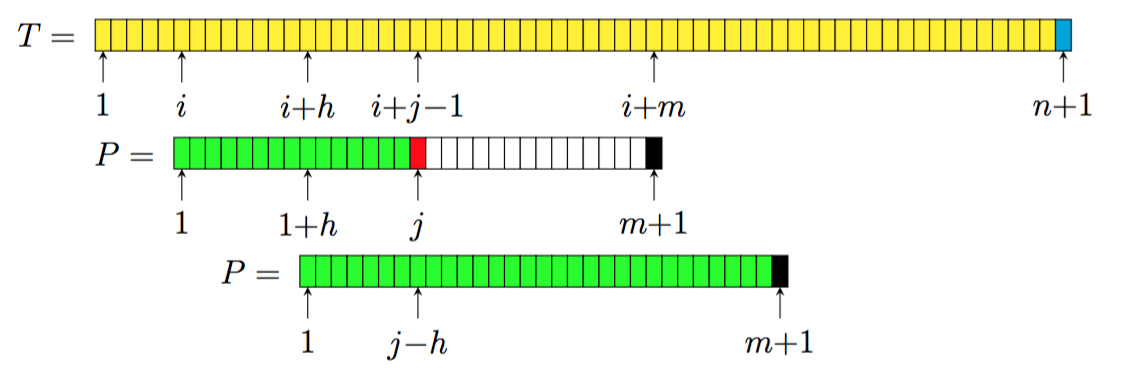
\includegraphics[width=.8\textwidth]{./notes/immagini/l13-fig1.png}
\caption{Spostamento del pattern dopo è stato trovato un mismatch tra \textit{P[j]} e \textit{T[i+j-1]}}
\end{figure}

Durante l'esecuzione dell'algoritmo, si ha che il pattern \textit{P} è allineato al carattere \textit{i} della stringa e che ci sia un match parziale del pattern, ovvero che \textit{P[1, j-1] = T[i, i + j-2]} con un mismatch tra \textit{P[j]} e \textit{T[i+j-1]}. 

Risulta quindi necessario riallineare il pattern con un altro carattere della stringa, per cercare una nuova occorrenza completa (supponendo che questa ci sia).

Supponendo che ci sia un'occorrenza del pattern completa a partire da \emph{i+h} con $ 1 \leq h \leq j-1$, è necessario che $P[1, j-h-1]$ siano uguali a $P[1+h, j-1]$, inoltre, $P[j-h]$ deve essere diverso di
$P[j]$, perché è già stato fatto un confronto tra $P[j]$ e $T[i+j-1]$, e sono stati trovati diversi.

Questo vuol dire che il prefisso $P[1, j-h-1]$ deve comparire all'interno del pattern, in particolare si ha che $\pi_{1+h} = j - h -1$, ovvero $j = \pi_{1+h} +h +1$.

Pertanto gli spostamenti \textit{h} compresi tra 1 e \textit{j-1} per i quali può esserci un'occorrenza del' pattern in posizione \textit{i+h} sono solamente quelli per cui $j = \pi_{1+h} +h +1$.
Se questa condizione non è soddisfatta per nessun \textit{h}, la prima posizione del testo in cui può esserci una occorrenza del pattern è \textit{i+j}.

$$
min(\{j\} \cup \{h | 1 <= h < j, j = 1 + h + \pi_{1+h}^P\})
$$

Nel caso venga trovato un match del pattern, si ha un mismatch sul
carattere \emph{j=m+1} perché è la sentinella, in questo caso lo
spostamento equivale al periodo minimo della stringa \emph{P}:

$$
d[m+1] = min(\{m+1\} \cup \{h | 1 \leq h \leq m, m+1 = 1 + h + \pi_{1+h}^S\})
$$

Se \emph{h = m}, ovvero la stringa non è periodica, si ha che viene
preso in considerazione il periodo degenere, che è pari alla lunghezza
della stringa, quindi anche nel caso di un match completo si ottiene lo
spostamento corretto.

Per calcolare $d[j]$ si può utilizzare

\begin{breakablealgorithm}
	\begin{algorithmic}[1]
		\For{$ j = 1 \: \text{to} \: m +1 $}
			\State // Diamo ad ogni \textit{d[j]} il valore \textit{j} che è il massimo dei valori tra cui minimizzare
			\State $ d[j] = j $
		\EndFor
		\For{$ h = m \: \text{downto} \: 1 $}
			\State // Aggiorniamo d[j] quando troviamo un h minore che soddisfa la condizione $j = 1 + h + \pi_{1+h} $
			\State $ d[1 + h + pref[1+h]] = h $
	    \EndFor
	\end{algorithmic}
\end{breakablealgorithm}

Il tutto viene fatto in \emph{O(m)}, perché viene scorso 2 volte il
pattern.

L'algoritmo risulta quindi essere:

\begin{breakablealgorithm}
	\caption{KMP: Algorimto di Knuth-Morris-Pratt}
	\begin{algorithmic}[1]
	\Function{Knuth-Morris-Pratt}{$ P,Y $})
    \State $ pref \gets \text{\textsc{Funzione-Prefisso}}(P) $
    \For{$ j = 1 \text{ to } m+1 $}
		\State $ d[j] \gets j $
	\EndFor
    \For{$ h = m \: \text{downto} \: 1 $}
	    \State $ d[1 + h + pref[1+h]] = h $
    \EndFor
	\State $ i,j \gets 1 $
    \While{$ i \leq n - m +1 $}
        \While{ $ P[j] = T[i+j-1] $}
            \State $ j \gets j + 1 $
        \EndWhile
        \If{$ j > m $}
            \State// Segnala occorrenza in posizione \textit{i}
        \EndIf
        \State $ i \gets i + d[j] $ \Comment{Spostamento nella stringa T}
        \State $ j \gets \max(1, j - d[j]) $ \Comment{Spostamento interno al pattern}
	 \EndWhile
	 \EndFunction
	\end{algorithmic}
\end{breakablealgorithm}

\subsubsection{Complessità dell'algoritmo}\label{complessituxe0-dellalgoritmo}

La complessità della funzione prefisso e dei due cicli \texttt{for}
risulta essere \emph{O(m)}.

Durante la ricerca, l'operazione che viene effettuata più volte è il test del ciclo \texttt{while} interno. 
Se il confronto ha esito negativo, il pattern viene ri-allineato e le posizioni possibili in cui è possibile allineare il pattern sono \emph{n - m +1}, quindi possono essere fatti al massimo \emph{n - m +1} confronti con esito negativo.

Quando il confronto ha esito positivo, \emph{i + j - 1} non diminuisce mai e aumenta di uno se viene trovato un match. Dal momento che, all'inizio \emph{i + j - 1 = 1} e alla fine vale $i + j -1\leq n+1$, perché
deve essere un carattere della stringa \emph{T} o al più la sentinella.

Segue che al massimo il numero di match è $\leq n + 1 - 1$.

Considerando sia i match che i mismatch, si hanno al massimo $2n-m+1$ confronti e considerando l'\emph{O(m)} iniziale, si ha come
complessità totale dell'algoritmo \emph{O(m+n)}.

\subsection{Algoritmo di Boyer e Moore}\label{algoritmo-di-boyer-e-moore}

Quando viene allineato il pattern con il testo i confronti dei
caratteri vengono effettuati a partire dalla fine del pattern, andando a
ritroso.

Lo svantaggio di questo algoritmo è che nel caso peggiore, vengono fatti
\emph{4n} confronti, tuttavia nel caso ottimo l'algoritmo riesce a
confrontare un numero di caratteri $\leq n$.

Dal momento che l'approccio utilizzato va a ritroso, la sentinella viene
aggiunta all'inizio, sia del pattern che del testo, nella posizione 0.

\begin{figure}[htbp]
\centering
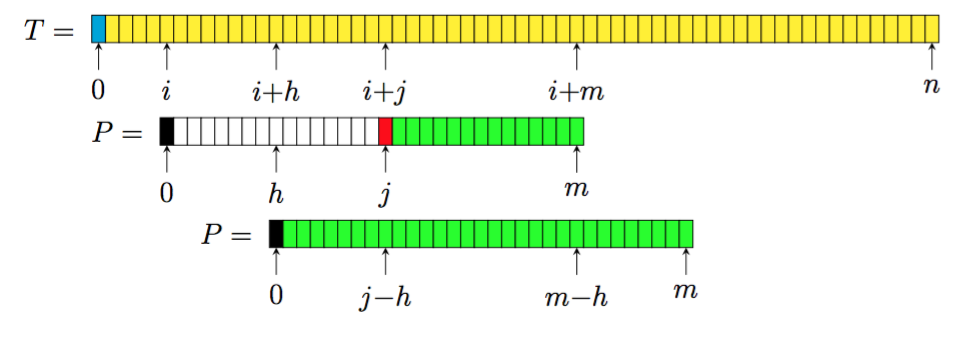
\includegraphics[width=.8\textwidth]{./notes/immagini/l13-fig2.png}
\caption{Spostamento con $ 1 \leq h \leq j-1 $}
\end{figure}

Con la sentinella $P[0]$ allineata con il carattere $T[i+j]$ e partendo dal fondo si è trovato un primo mismatch in posizione \emph{j}, vi è una occorrenza del pattern quando la
sentinella è allineata con $T[i+h]$ per uno spostamento
\emph{h} compreso tra 1 e \emph{j-1}

Siccome l'algoritmo confronta i caratteri da destra a sinistra sappiamo
che ad un certo punto

$$
P[j + 1, m] = T[i + j + 1, i + m] \text{ e che } P[j] \neq T[i + j]
$$

Supponiamo che ci sia un'occorrenza del pattern a partire da $ T[i+h+1] $, ovvero quando la sentinella \textit{P[0]} è allineata con $ T[i+h] $ per un certo spostamento $ 1 \leq h \leq j -1 $.

In questo caso si ha che

$$
P[j-h, m-h] = T[i+j,i+m]
$$

e dal momento che c'è un match parziale a partire da \textit{i}, ovvero che$ P[j + 1, m] =  T[i + j + 1, i + m]$, si ha che 

$$
P[j - h +1,m -h] = T[i+j+1, i+m]  = P[j+1,m]
$$

In altre parole, dal momento che la sottostringa $ T[i+j+1, i+m] $ matcha sia con la terminazione del pattern ($ P[j+1,m] $), sia con la parte centrale del pattern $ P[j - h +1,m -h] $, la parte centrale del pattern è uguale a quella terminale.

Inoltre, dato che $ P[j] \neq T[i+j] $, $ P[j] $ è anche diverso da $ P[j-h] $, perché quando il pattern è allineato su $ i+j $ c'è un match e quindi $ P[j-h] = T[i+j] $.

Sia $ P_{rev} $ la stringa ottenuta rovesciando il pattern \textit{P}, ovvero se $ P = x_0,x_1,\ldots , x_m $ allora $ P_{rev} = x_m, \ldots, x_1, x_0 $\footnote{Non è necessario costruire la stringa $ P_{rev} $ dal momento che serve solo per la funzione prefisso. Viene utilizzata solamente per facilitare l'esposizione}.

Per costruzione si ha che

$$
P[j-h +1, m-h] = P[j+1,m] \Rightarrow P_{rev}[1+h, m-j+h] = P_{rev}[1,m-j]
$$

e che

$$
P[j-h] \neq P[j] \Rightarrow P_{rev}[m-j+h+1] \neq P_{rev}[m-j+1]
$$

Ma questo vuol dire che in $ P_{rev}[1+h] $ inizia l'occorrenza del prefisso $ P_{rev}[1,m-j] $, pertanto $\pi_{1+h}^{P_{rev}} = m -j$, ovvero che 

$$
j = m - \pi_{1+h}^{P_{rev}} 
$$

Pertanto, gli spostamenti \textit{h} compresi tra 1 e \textit{j - 1} tali che ci possa essere una occorrenza del pattern quando $ P[0] $ è allineato con $ T[i+h] $ sono soltanto quelli per cui $ j = m - \pi_{1+h}^{P_{rev}} $.

Supponiamo invece che l'occorrenza del pattern ci sia per uno spostamento $ j \leq h leq m $.

\begin{figure}[htbp]
	\centering
	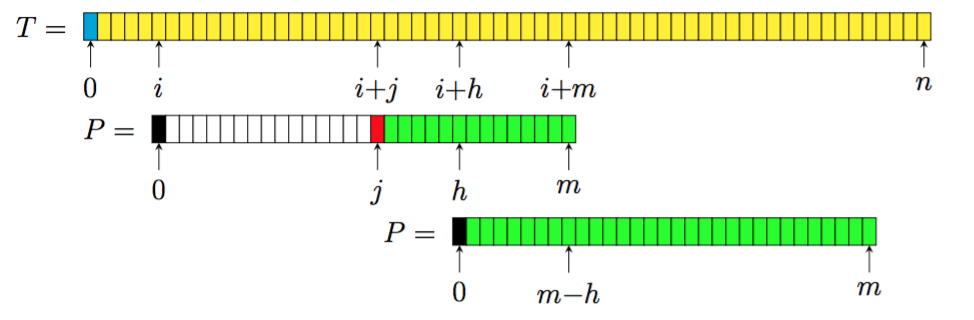
\includegraphics[width=.8\textwidth]{./notes/immagini/l13-fig3.png}
	\caption{Spostamento con $ j \leq h \leq m $}
\end{figure}

In questo caso si ha 

$$
P[1,m-h] = T[i+h +1, i+m]
$$

e siccome $ P[j+1,m] = T[ièj+1,i+m] $ dovrà essere che

$$
P[h+1,m] = P[1,m-h]
$$

Ovvero il pattern \textit{P}, e quindi anche $ P_{rev} $, ha un bordo di lunghezza $ m-h $ e questo equivale a dire che $ \pi_{1+h}^{P_{rev}} = m-h $.

Pertanto gli spostamenti \textit{h} compresi tra \textit{j} e \textit{m} tali che ci possa essere un'occorrenza del pattern sono soltanto quelli per cui $ \pi_{1+h}^{P_{rev}}  = m-h $.

Si ha quindi che lo spostamento $d[j]$ del pattern che si deve effettuare quando, con la sentinella allineata ala carattere $ T[i] $ del testo e partendo dalla fine del pattern si trova un mismatch tra il carattere $ P[j] $ e $ T[i+j] $ è:

$$
d[j] = min(\{h | 1 \leq h < j, j ) m , \pi_{1+h}^{P_{rev}}\} \cup \{h | j \leq h \leq m, h = m - \pi_{1+h}^{P_{rev}}\})
$$

Tale minimo è sempre definito perché \emph{h = m} soddisfa sempre la seconda condizione, dal momento che $ \pi_{1+m}^{P_{rev}}  = 0$ perché il carattere $ P_{rev}[m+1] $ è la sentinella.
